\documentclass[12pt]{article}

\usepackage{amsmath, amssymb}
\usepackage{geometry}
\usepackage{setspace}
\usepackage{graphicx}
\usepackage[hidelinks]{hyperref}
\usepackage{tikz}
\usetikzlibrary{calc}

\geometry{margin=1in}
\onehalfspacing

\title{\textbf{An Algebraic Translation of Newton's Proposition XI}\\
\large From \emph{Philosophiæ Naturalis Principia Mathematica}, Book I}
\author{Mohamed Ahmed}
\date{}

\begin{document}
\maketitle

\noindent\textbf{Course:} Newton's Principia\\
\textbf{Instructor:} Andrew Mclntyre

\vspace{0.3in}

\section*{Introduction}

In Book I of Isaac Newton's \emph{Philosophiæ Naturalis Principia Mathematica}, there are series of propositions. Proposition XI is one of the important propositions and it tells us that a body moving along an elliptical orbit is driven by a centripetal force that is directed toward a focus of the ellipse. The question is: what is the law that tells us how strong this force is? Newton's original proof uses only geometry. He uses ratios of lines, limits of polygons, and arguments about curvature. He does not use algebra or calculus.

The goal of this project is to take Newton's geometric reasoning and write it in modern algebraic language and as well as explain it in natural language. But I want to keep the same logical structure of Newton's argument. I will not assume any force law from the beginning. Instead, my goal is to find the inverse-square law by using results that Newton already proved earlier in Book I.

\section*{Statement of Proposition XI (Newton)}

\begin{quote}
\emph{Let a body revolve in an ellipse; it is required to find the law of the centripetal force tending toward a focus of the ellipse.}
\end{quote}

Let me break down what this statement tells us. First, the path of the body (any object) is an ellipse. Second, the force is always directed toward one of the foci of the ellipse. Third, the body continues its motion along the curved path of the ellipse. Given these facts, Newton wants to determine exactly how strong this centripetal force must be.

Newton's conclusion is that the centripetal force is inversely proportional to the square of the distance from the focus. This means that when the distance from focus to point $P$ gets bigger, the force gets smaller, and the force gets smaller by the square of the distance.

\section*{Prior Results Used by Newton}

Newton's proof of Proposition XI uses propositions already proved before prop. 11. So I will re-state these first before I use them in the proof of Proposition XI.

\subsection*{Proposition I (The Area Law)}

From Proposition I, I learned that if a body is under the influence of a centripetal force, then the radius drawn from the force center sweeps out equal areas in equal times. In other words, the object covers equal areas in equal times.

To write this down mathematically, I need a way to measure how fast the area is being swept out. In modern calculus, I can find the velocity at which the area is changing. This rate of change has a special name. It is called the \emph{areal velocity}. Proposition I tells us that this areal velocity is constant. I can write this as:
\[
\frac{dA}{dt} = \text{constant}.
\]

Now, I need to connect this to the motion of the body. To do this, I need to relate the swept area to where the body is located. I can describe where the body is using polar coordinates. In polar coordinates, $r$ is the distance from the force center, and $\theta$ is the angle measured from some reference direction. 

When the body moves just a tiny bit, the radius vector sweeps out a small area. In polar coordinates, this small area is approximately equal to $\frac{1}{2}r^2 d\theta$. I can think of it like a thin triangular slice. The rate at which the angle changes is $\dot{\theta} = \frac{d\theta}{dt}$. So now the areal velocity becomes:
\[
\frac{dA}{dt} = \frac{1}{2}r^2 \dot{\theta}.
\]

Since the areal velocity is constant, and the factor of $\frac{1}{2}$ is just a constant number, this means that $r^2 \dot{\theta}$ must also be constant. I can write this as:
\[
r^{2}\dot{\theta} = h,
\]
where $h$ is just a constant. This relationship is very important. I will need it later when I connect the geometry of the ellipse to the force law.

\subsection*{Proposition VI (Force and Sagitta)}

From Proposition VI, I learned about what happens when I take really small steps along the path. If I move really small steps along the path of the object, following the tangent, I will have really small deviations from the path. These deviations happen because of the centripetal force. Newton shows that the centripetal force is proportional to those small deviations from the path. Newton calls these small deviations the \emph{sagitta}.

To be more precise, Newton looks at an infinitesimally small arc of a curve. He compares it to the straight-line motion along the tangent. The perpendicular deviation of the curve from the tangent is what he calls the \emph{sagitta}. Newton proves that the centripetal force at the midpoint of the arc is proportional to the sagitta. Also, it is inversely proportional to the square of the tine elapsed.

In algebraic form, I can write this as:
\[
F \propto \frac{\text{sagitta}}{(\Delta t)^2}.
\]

Since displacement due to force grows like time squared, this relation tells me that force is proportional to the curvature of the path.

\section*{Geometric Properties of the Ellipse}

Let me consider an ellipse to visualize. This ellipse has a semi-major axis $a$ and a semi-minor axis $b$. Let $S$ be one focus of the ellipse. Let $P$ be a point on the ellipse. The distance from $S$ to $P$, which is $SP$, I will call $r$. The ellipse has something called the \emph{principal latus rectum}. This is a constant that we will call $L$. It is given by the formula:
\[
L = \frac{2b^{2}}{a}.
\]

For more information about the properties of ellipses, this was helpful: click \href{https://byjus.com/jee/properties-of-ellipse/}{Properties of Ellipse}.

\begin{figure}[h]
\centering
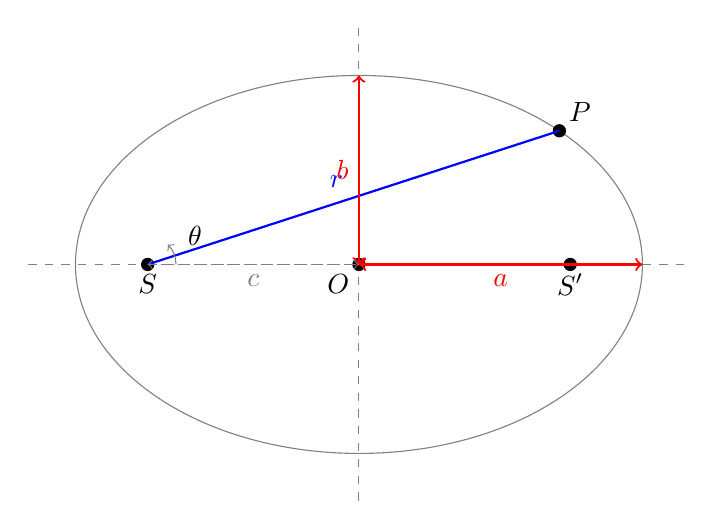
\begin{tikzpicture}[scale=1.2]
    % Define ellipse parameters
    \pgfmathsetmacro{\a}{3}      % semi-major axis
    \pgfmathsetmacro{\b}{2}      % semi-minor axis
    \pgfmathsetmacro{\c}{sqrt(\a*\a - \b*\b)}  % focal distance
    
    % Draw ellipse
    \draw[thin, gray] (0,0) ellipse ({\a} and {\b});
    
    % Draw axes
    \draw[dashed, gray] (-\a-0.5,0) -- (\a+0.5,0);
    \draw[dashed, gray] (0,-\b-0.5) -- (0,\b+0.5);
    
    % Mark center
    \fill (0,0) circle (2pt) node[below left] {$O$};
    
    % Mark foci
    \fill ({-\c},0) circle (2pt) node[below] {$S$};
    \fill ({\c},0) circle (2pt) node[below] {$S'$};
    
    % Mark a point P on the ellipse (upper right quadrant, angle ~45 degrees)
    \pgfmathsetmacro{\angle}{45}
    \pgfmathsetmacro{\px}{\a*cos(\angle)}
    \pgfmathsetmacro{\py}{\b*sin(\angle)}
    \coordinate (P) at (\px,\py);
    \fill (P) circle (2pt) node[above right] {$P$};
    
    % Draw line from focus S to point P
    \draw[thick, blue] ({-\c},0) -- (P) node[midway, above left] {$r$};
    
    % Draw semi-major axis
    \draw[<->, red, thick] (0,0) -- (\a,0) node[midway, below] {$a$};
    
    % Draw semi-minor axis
    \draw[<->, red, thick] (0,0) -- (0,\b) node[midway, left] {$b$};
    
    % Add labels for foci distance
    \draw[<->, gray, dashed] ({-\c},0) -- (0,0) node[midway, below] {$c$};
    
    % Add angle indicator at focus S
    \draw[->, gray] ({-\c+0.3},0) arc (0:\angle:0.3);
    \node at ({-\c+0.5},0.3) {$\theta$};
\end{tikzpicture}
\caption{An ellipse with focus $S$, center $O$, and a point $P$ on the ellipse. The distance from the focus to point $P$ is $r = SP$. The semi-major axis is $a$ and the semi-minor axis is $b$.}
\end{figure}

Newton uses this geometric constant $L$ to relate curvature properties of the ellipse to distances measured from the focus. This will help me understand how the ellipse curves at different points.

\section*{Curvature and the Sagitta}

For an infinitesimally small arc near point $P$, Newton shows something important. He uses similar triangles and limiting arguments to show this. What he shows is that the sagitta of the arc is proportional to
\[
\frac{r^{2}}{L}.
\]

This proportionality tells me how sharply the ellipse curves at different distances from the focus. When points are farther from the focus, the curvature is smaller. When points are closer to the focus, the curvature is greater.

\section*{Combining Geometry with Proposition VI}

From Proposition VI, I know that the centripetal force satisfies
\[
F \propto \frac{\text{sagitta}}{(\Delta t)^2}.
\]

Now I can substitute the geometric relation for the sagitta. When I do this, I get
\[
F \propto \frac{r^{2}}{L(\Delta t)^2}.
\]

However, I also know from Proposition I that the areal velocity is constant. This means that for an infinitesimal arc,
\[
\Delta t \propto r.
\]

So if $\Delta t$ is proportional to $r$, then
\[
(\Delta t)^2 \propto r^2.
\]

Now I can substitute this into the force expression. When I do this, I get
\[
F \propto \frac{r^{2}}{L r^{2}} = \frac{1}{L}.
\]

Since $L$ is constant for a given ellipse, this shows me something important. The force scales inversely with the square of the distance. In other words:
\[
F \propto \frac{1}{r^2}.
\]

\section*{Conclusion}

By translating Newton's geometric reasoning into algebraic proportionalities, I get back his result. The result is this: if a body is moving in an elliptical orbit under a centripetal force directed toward a focus, then it must be subject to a force that is inversely proportional to the square of its distance from that focus. This derivation uses only results that Newton had already established. These are the area law and the relationship between force and curvature. I did not introduce any modern physical assumptions.

This project shows how Newton's geometric arguments come before later algebraic formulations of classical mechanics. It also shows how modern notation can make the structure of his reasoning clearer. But the modern notation does not change what he was actually saying.

\end{document}
